
\chapter{Slackware包管理}
\label{chap:packageManagement}
\begin{flushleft}
\rule[0mm]{\textwidth}{.1pt}
\end{flushleft}

包管理在每个发行版中都是一个核心的问题。而所谓的软件包指的是一堆随时可
以安装的相关程序。一般情况下,我们是先下载一个源码包,将其解压、设置、
编译,最后再手工安装。而对于软件包,已经事先进行了这些步骤,所以我们只
要安装它就可以了。所以软件包可以认为是一堆事先编译好的二进制文件,将这
些文件打包压缩后就是所谓的软件包了。不需要自己编译是软件包的一大好外,
另一个好处就是可以方便地安装和卸载。Slackware自带了一套方便的包管理器。
有了它们,我们就可以很容易地制作软件包,对软件包进行安装、卸载及升级。

自从RedHat有了RPM包管理器后,人们就有一种说法,说Slackware没有包管理工
具。这显然太荒谬了。Slackware的包管理工具一直存在,甚至在RedHat发行版
出现之前就有了。当然,功能可能不如rpm包管理器(同样适用于deb包),或者
不如它存在普遍,但\texttt{pkgtool}及相关的程序在安装如rpm等包的功能上毫
不逊色。关于那个说法的真实情况并不是指\texttt{pkgtool}不存在,而是指
\texttt{pkgtool}不解决包的依赖关系。

很自然地,包管理器在很多Linux社区用户的脑中,就必须是包含解决依赖的功
能。好吧,现在你知道了,这并不是那么地``理所当然''。这并不是说
Slackware的包没有依赖关系,而是指这些包管理软件并不对依赖进行检查。依
赖管理则交由系统管理员解决,这是种很好的方式,不管你信不信,我反正是信
了。

\section{Slackware的包格式}
\label{sec:packageManagement:format}
在学习这些包管理工具之前,我们要先熟悉Slackware的包格式,在Slackware中,
一个软件包只是一个使用\texttt{gzip}压缩的软件包。而安装一个包只是简单
地将它解压到根目录下。

下面是我们虚构的一个软件及其对应的软件包:
\begin{Verbatim}[frame=single, commandchars=\\\{\}]
./
usr/
usr/bin/
usr/bin/makehejaz
usr/doc/
usr/doc/makehejaz-1.0/
usr/doc/makehejaz-1.0/COPYING
usr/doc/makehejaz-1.0/README
usr/man/
usr/man/man1
usr/man/man1/makehejaz.1.gz
install/
install/doinst.sh
\end{Verbatim}
要安装这个包,包管理系统会将这些文件解压到根目录下。而包数据库中会创建
一个新的条目,以便之后用于升级或删除这个包。条目的内容就是这些文件的路
径。

要注意\path{install/}子目录,这是一个特殊的目录,因为它包含了一个特殊
的脚本文件:\path{doinst.sh},如果包管理系统发现有这个文件,在安装结束
后会执行该脚本,以对软件做一些安装后的设置工作。

包中也可以包含一些其它的脚本,在
\ref{sec:packageManagement:makingPackages:makepkg}会详细介绍。

\section{包管理工具}
\label{sec:packageManagement:utilities}
Slackware主要包括四个包管理工具,分别执行软件包的安装、卸载及升级。

\subsection{pkgtool}
\label{sec:packageManagement:utilities:pkgtool}
\texttt{pkgtool}(8)是一个菜单驱动的程序,它的作用是安装、卸载软件包。
主菜单如图\ref{fig:pkgtool}显示。
\begin{figure}[htpb]
  \centering
  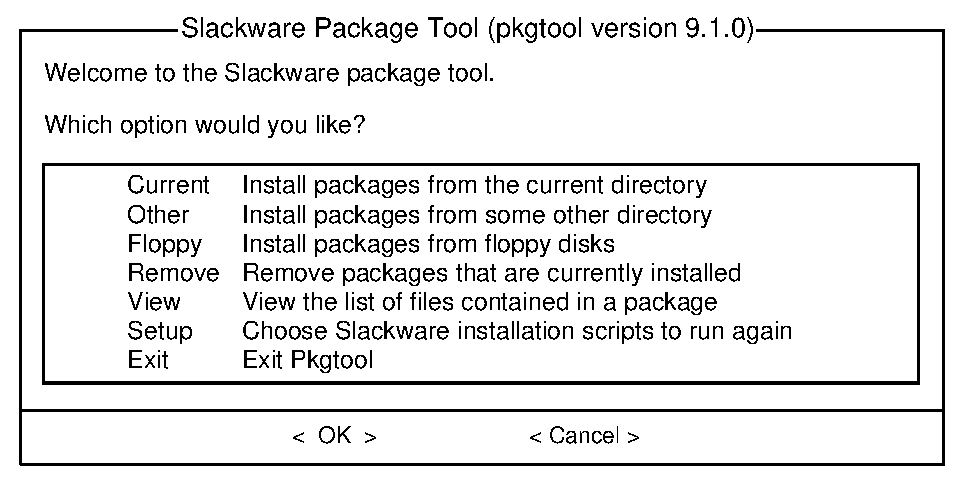
\includegraphics[width=0.8\textwidth]{images/package-management/pkgtool.eps}
  \caption{Pkgtool主界面}
  \label{fig:pkgtool}
\end{figure}
使用该工具,可以对当前目录或其它目录下的软件包进行安装。只要选择希望使
用的安装方式,pkgtool就会在相应的位置寻找可以安装的软件包。之后可以看
到可安装软件包的一个列表,如图\ref{fig:pkgtool-view}所示。
\begin{figure}[htpb]
  \centering
  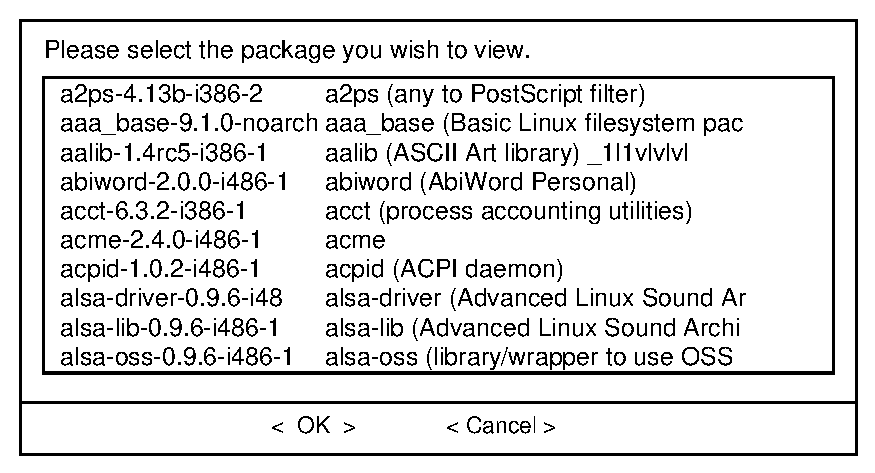
\includegraphics[width=0.8\textwidth]{images/package-management/pkgtool-view.eps}
  \caption{pkgtool的View模式}
  \label{fig:pkgtool-view}
\end{figure}
如果你想删除软件包,那么选择remove选项,就会出现所有已安装软件包的清单。
只要标记那些想删除的包,之后点OK就可以了。\texttt{pkgtool}会卸载它们。

另一些用户喜欢使用命令行工具。当然,你也应该知道,命令行工具提供了更多
的选项。另外,升级软件包的功能只能由命令行工具实现。

\subsection{installpkg}
\label{sec:packageManagement:utilities:installpkg}
\texttt{installpkg}(8)为系统处理安装新软件包的任务。语法如下:
\begin{Verbatim}[frame=single, commandchars=\\\{\}]
# \textbf{installpkg option package_name}
\end{Verbatim}
\texttt{installpkg}有三个选项,一次只能使用一个选项。
\begin{table}[htpb]
  \centering
  \begin{tabular}{c|l}
    \hline\hline 
    选项 & 作用 \\ \hline
    -m & 在当前文件夹下执行makepkg。 \\
    -warn & \parbox[t]{12cm}{在安装前显示如果安装后会发生的变化,这个选项对于用于生
    产的系统较为有用。它能在安装前让用户知道安装后系统的变化。} \\
    -r & \parbox[t]{12cm}{递归安装当前文件夹及其子文件夹中的软件包。指定软件包时可以使
    用通配符,那么在搜索时会用该通配符进行匹配。}\\
    \hline
  \end{tabular}
  \caption{installpkg选项}
  \label{tab:installpkg-option}
\end{table}

如果在\texttt{installpkg}之前传递了\texttt{ROOT}环境变量,则
\texttt{installpkg}会使用该变量中的路径作为根目录。这对于为安装新的系
统或为设置其它磁盘上的Slackware来说很有用。一般可以将它们挂载到
\path{/mnt}或其它是不\path{/}的目录下。

已安装的软件包数据库条目存储在\path{/var/log/packages}目录下。每个条目
都只是一个纯文本文件,一个软件包对应一个文件。如果一个软件包包含了安装
后执行的脚本文件,那么它会被存储在\path{/var/log/scripts/}目录中。

我们可以为\texttt{installpkg}执行几个软件包或是使用通配符。注意,
\texttt{installpkg}在覆盖一个软件包时不会有任何提示。所以如果你想确保
旧软件包的文件被正确删除,那么请使用\texttt{upgradepkg}。

\subsection{removepkg}
\label{sec:packageManagement:utilities:removepkg}
\texttt{removepkg}(8)用来卸载系统上的某个软件包。语法如下:
\begin{Verbatim}[frame=single, commandchars=\\\{\}]
# \textbf{removepkg option package_name}
\end{Verbatim}
\texttt{removepkg}有四个选项,一次只能使用一个选项。
\begin{table}[htpb]
  \centering
  \begin{tabular}{c|l}
    \hline \hline
    选项 & 作用 \\ \hline
    -copy & \parbox[t]{12cm}{该软件包会被复制到一个预留的软件包目录。使
      用该选项不会删除原来的包,它是是创建一个新的软件包树。}\\
    -keep & \parbox[t]{12cm}{保存删除过程中的缓存文件。这个选项只对调
      试有用。} \\
    -preserve & \parbox[t]{12cm}{删除软件包,同时将其复制到预留的目录
      下。}\\
    -warn & \parbox[t]{12cm}{告诉我们如果删除软件包,会发生什么
      (removepkg的行为)。}\\
    \hline\hline
  \end{tabular}
  \caption{removepkg选项}
  \label{tab:removepkg-options}
\end{table}
与\texttt{installpkg}一样,可以为\texttt{removepkg}传递\texttt{ROOT}环
境变量。则\texttt{removepkg}会将该路径作为根目录进行操作。

\texttt{removepkg}会搜索已安装的软件包并只删除与指定文件名唯一匹配的那
个软件包。它还会搜索指定软件包的\texttt{doinit.sh}脚本,并删除由它创建
的所有符号链接。

在删除过程中,会显示一个状态报告。而在删除后,安装包数据库中对应的条目
会被移动到\path{/var/log/removed_packages}目录中,而对应的
postinstall\footnote{不知道怎么翻译这个词}脚本则会被移动到
\path{/var/log/removed_scripts}目录中。

与\texttt{installpkg}相同,我们可以同时指定多个软件包,或使用通配符来
表示软件包的名称。

\subsection{upgradepkg}
\label{sec:packageManagement:utilities:upgradepkg}
\texttt{upgradepkg}(8)的作用是用更新软件包,语法如下:
\begin{Verbatim}[frame=single, commandchars=\\\{\}]
# \textbf{upgradepkg package\_name}
或
# \textbf{upgradepkg old\_package\_name\%new\_package\_name}
\end{Verbatim}
\texttt{upgradepkg}的工作方式是先安装新的软件包,再删除旧的软件包,那
样旧的软件包就不再存在于系统中。如果更新后的软件包名称变化了,则使用百
分号(`\%')来指定已安装的旧软件包的名称(上述第二种方式)和新软件包的名
称。

同样可以为\texttt{upgradepkg}传递\texttt{ROOT}环境变量。

\texttt{upgradepkg}不是完美的,所以在更新之前请自己保存配置文件。如果
更新后覆盖了这些文件,而最后又不能使用,那就需要之前的备份来进行恢复。

和\texttt{installpkg}和\texttt{removepkg}一样,可以一次指定多个软件包,
也可以使用通配符来表示软件包名称。

\subsection{rpm2tgz/rpm2targz}
\label{sec:packageManagement:utilities:rpm2}
由于RedHat的包管理器很流行,许多软件包就是以RPM的形式发行的,由于这不
是Slackware原生的包,所以建议不要依赖它们,但有时,我们只能得到RPM格式
的文件(甚至是源码)。

所以我们提供了一个程序,能将RPM包转化为Slackware原生的\texttt{.tgz}格
式。这就使我们能将它解压到一个临时文件夹中(可以使用
\texttt{explodepkg})并检查它的内容。

\texttt{rpm2tgz}程序会以\texttt{.tgz}的扩展名创建Slackware包,而
\texttt{rmp2targz}则是将RPM包转为一个以\texttt{.tar.gz}为扩展名的归档
文件。

\section{制作软件包}
\label{sec:packageManagement:makingPackages}
制作Slackware的软件包说难则难,说简单也简单。首先,没有一个标准的制作
包的方法。唯一的要求是最后要是一个用tar打包、gzip压缩(现在鼓励使用xz)
的文件,如果还有postinstallation脚本的话,就只能是
\path{/install/doinst.sh}。

如果你对制作软件包感兴趣,那么我们建议你看看Slackware源码树中的创建脚
本。我们可以使用几种方式创建软件包。


\subsection{explodepkg}
\label{sec:packageManagement:makingPackages:explodepkg}
\texttt{explodepkg}(8)的作用与\texttt{installpkg}类似,它们都是解压一
个软件包,但不同的是,\texttt{explodepkg}并不执行安装,也不在安装数据
库中记录,而只是将软件包解压到当前文件夹中。

如果你查看了Slackware的源码树,那么你就会看到我们如何将该命令运用到
``framework''软件包中,这些包的内容和软件包的最终结构很像,它们包含了
所有的文件名(内容是空的)、权限即所属。而创建脚本只是将这个包的内容从
软件包解压到软件包的构建目录中。

\subsection{makepkg}
\label{sec:packageManagement:makingPackages:makepkg}
\texttt{makepkg}(8)会将当前目录的内容打包为一个有效的Slackware包。它会
搜索当前目录的符号链接,并将这些符号链接转化为一系统的ln命令存放在
\texttt{doinit.sh}脚本中,然后删除符号链接。如果遇到空的文件(长度为0),
它也会发出警告。

一般而言,这个命令是在我们构建好软件包树后运行的。

\subsection{SlackBuild脚本}
\label{sec:packageManagement:makingPackages:slackbuild}
出于需要,Slackware的软件包是由不同方式构建的。而并不是所有的软件包都
是用同一种方式写的,因此编译的方式也不同。而许多编译时的选项在
Slackware的包中并不包括。而如果我们需要使用这些选项,我们就必须自己编
译它。幸运的是,许多的Slackware源码树中的包都有一个SlackBuild脚本。

那什么是SlackBuild脚本呢?SlackBuild脚本是一个以\texttt{root}执行的脚
本,它会自动解压源码包,对其进行配置、编译,并最终创建对应的Slackware
包。我们可以自由地修改源码目录下的这些脚本,创建自己的Slackware包。

还有,现在有一个网站\url{http://slackbuilds.org},上面包含了许多主流软
件的SlackBuild脚本。通过它我们就能很方便地创建和安装软件包。

\section{创建Tags和Tagfiles(用于setup程序)}
\label{sec:packageManagement:tagfile}
还记得安装Slackware时有一种方式是从tagfile安装吗?Slackware的setup程序
只是处理要安装到系统的软件包,而tagfile就是用来告诉setup程序哪些必须安
装、哪些是可选的,哪些是默认勾选的。

tagfile文件存放在第一个软件包系统中的,它列出了一个特定系列中软件包的
安装状态。这些状态有:
\begin{table}[htpb]
  \centering
  \begin{tabular}{c|l}
    \hline \hline
    选项 & 含义 \\ \hline
    ADD & 表示要正常运作系统必要的软件包。\\
    SKP & 安装过程会跳过该软件包。\\
    REC & 不是必要的,但推荐安装。\\
    OPT & 该包为可选的。\\
    \hline\hline
  \end{tabular}
  \caption{tagfile状态选项}
  \label{tab:tagfile-options}
\end{table}

而tagfile文件中的每一行则为一个软件包和对应的状态:
\begin{Verbatim}[frame=single, commandchars=\\\{\}]
package_name: status
\end{Verbatim}
在Slackware DVD中,tagfile是存放于每个软件系列的目录下,名为
\texttt{tagfile}。所以如果你的tagfile弄乱了,可以重新使用这个。

许多系统管理员习惯创建自己的tagfile,运行安装器,并选择``full''选项。
setup程序会读取每一个tagfile,并根据其中的内容安装软件包。如果你使用了
\texttt{REC}或\texttt{OPT}状态,则\texttt{setup}会显示一个窗口,询问是
否安装它。因此,如果想要自动安装,我们建议你使用\texttt{ADD}及
\texttt{SKP}。

切记,请确定你的tagfile与原来的tagfile存在于同一目录下,或者可以在安装
时指定自己的tagfile的位置。

%%% Local Variables: 
%%% mode: latex
%%% TeX-master: "../SlackGuide"
%%% End: 
